\section{PoD Consensus Algorithm}
\label{sec:pod}

\subsection{Design Goals}
\label{pod:goals}

The consensus algorithm is one of the cornerstones of blockchains, and its rapidity and irreversibility are our focus. In addition, in order to build a good ecology of Nebulas, we believe that fairness is equally important. If the big capital can easily gain power to control the block consensus in Nebulas, the interests of many developers and users will be damaged. It is difficult for an ecology which cannot guarantee the interests of contributors to create in-depth value, as it goes against the design principles of Nebulas. Thus, the consensus algorithm should be designed to ensure the rapidity and irreversibility first, on which basis we will pursue fairness as much as possible, so as to guarantee the interests of contributors in Nebulas.

%共识算法作为区块链的基石之一,快速和不可逆是我们重点关注的目标。除此之外,为了更好地建设公链生态,我们认为公平性同样重要,如果大资本可以轻松占据公链中区块共识的话语权,那么会有很多公链上的开发者和用户的利益无端受损,一个不能保障公链建设者利益的生态,很难沉淀出价值深度,和星云链设计原则相违背。所以我们在设计共识算法时,在优先保证快速和不可逆的情况下,将尽可能追求公平性,维护公链建设者的利益。

\subsection{Defects of Commonly Used Consensus Algorithms}
\label{pod:weakness}

We have tried to find suitable commonly used consensus algorithms that match with our design goals, but these algorithms cannot completely meet our requirements.

%我们试图在较为常用的共识算法中找到符合我们设计目标的选择,但是这些算法和我们的目标多少都有些差距。

The PoW (Proof of Work) consensus algorithm is a zero-sum game, which uses the competitive hash calculation to determine the bookkeeper, rendering a great amount of electric power in the whole ecology wasted in the competition when any blocks are fed out, and thus the mining cost is high and the speed is restricted. With the increase of nodes involved in mining, the probability of each node to obtain the bookkeeping right will be reduced, leading to a continuous rise in the cost of stable feed-out of blocks under the PoW protocol. The Bitcoin, which continues to increase the difficulty of mining, has to face the situation sooner or later where the mining machine cannot make ends meet, while Ethereum has long been considering the use of the new PoS consensus algorithm Casper \cite{casper} to gradually replace the current PoW consensus \cite{buterin2013ethereum}. It can be seen that in view of the mining speed and the economic cost, the PoW is not beneficial to the long-term rapid development of the ecology of Nebulas, which is against our "rapid" goals.

%PoW (Proof of Work)工作量证明共识算法为零和博弈,采用竞争性哈希计算来确定记账人,导致了整个生态每次出块时都有大量电能在竞争中被无端消耗,挖矿成本高,而且速度受限。如果把公链参与者作为整体来看,随着参与挖矿的节点增加,每个节点获得记账权的概率将会减小,那么PoW协议下生态维持平稳出块的成本将会持续升高。不断增加挖矿难度的Bitcoin早晚需要面临矿机收益入不敷出的情形,而Ethereum则早已在考虑使用新的PoS共识算法Casper~\cite{casper}来逐步取代现阶段的PoW共识~\cite{buterin2013ethereum}。可见,从挖矿速度和经济成本角度,PoW都不利于公链生态的长期快速发展,和我们“快速”的目标不相符。

The PoS (Proof of Stake) consensus algorithm attempts to use the asset amount to replace the hash rate and distribute the probability of obtaining the bookkeeping right according to the coin age or deposit amount. Currently, both Peercoin \cite{king2012peercoin} and the Casper Protocol of Ethereum adopt the PoS consensus algorithm. This algorithm overcomes the shortcoming of the high power consumption of PoW but visually enlarges the impact of the capital on the probability distribution of the bookkeeping right. Compared with PoW, the big capital under PoS is more likely to gain power to control the ecology and form large group monopoly, possibly damaging the interests of the ecology contributors and impacting adversely on the value generation of Nebulas, all of which are against our "fairness" goal.

%PoS (Proof of Stake)股权证明共识算法试图采用资产的多寡来取代算力的作用,按照币龄或者押金数额来分配获得记账权的概率,现阶段Peercoin~\cite{king2012peercoin}和Ethereum的Casper协议都采用了PoS共识算法。这种算法解决了PoW高能耗的弊端,但很直观地放大了资本对记账权概率分配的影响,相较于PoW,在PoS下大资本更容易占据生态的话语权,形成大集团垄断,可能会对生态的建设者的利益造成损害,不利于公链生态的价值沉淀,同样和我们“公平性”的目标不相符。

The PoI (Proof of Importance) consensus algorithm was first proposed by Nem \cite{nem}. Different from PoS, the concept of account importance is introduced to PoI, and the account importance score is used to distribute the probability of the bookkeeping right. This algorithm overcomes the shortcoming of the high power consumption of PoW and relieves the PoS capital monopoly crisis, but exposes the "nothing-at-stake" problem. The cost for a cheater to reverse a block is significantly reduced, which goes against our "irreversibility" goal.

%PoI (Proof of Importance)重要度证明共识算法最早由Nem提出~\cite{nem},不同于PoS,PoI中引入了账户重要程度的概念,使用账户重要性评分来分配记账权的概率。这种算法解决了PoW的高能耗弊端,减缓了PoS的资本垄断危机,但暴露了nothing-at-stake的问题,作弊者逆转一个区块的成本被大大降低,和我们“不可逆”的目标不相符。

In short, in view of the discrepancy between commonly used consensus algorithms and our goals, we have proposed the PoD (Proof of Devotion) algorithm to integrate PoI, which evaluates the comprehensive account influence, with PoS, which involves strict economic penalties. PoS enhances the irreversibility of PoI, while PoI reversely contains the monopoly of PoS, which facilitates the free and rapid development of the ecology.

%综上,鉴于常用共识算法和我们目标存在差距,我们提出了基于账户贡献度的PoD (Proof of Devotion)算法,将评估账户综合影响力的PoI和具有严格经济惩罚的PoS相融合,利用PoS强化PoI的不可逆性,使用PoI反向遏制了PoS的垄断性,以此为生态自由快速发展助力。

\subsection{Design of the PoD Algorithm}
\label{pod:design}

\subsubsection{Generation of New Blocks}
\label{pod:design:block}

Similar to the PoI consensus algorithm that selects highly important accounts, the PoD selects the accounts with high influence in the ecology. The difference lies in that the PoD empowers the selected accounts to have the bookkeeping right with equal probability to participate in new block generation in order to prevent tilted probability that may bring about monopoly.

%类似PoI共识算法选取重要性高的账户,PoD将选取生态中贡献度较高的账户,不同之处在于,PoD赋予选取出来的账户平等概率的记账权来参与产生新区块 (block),防止概率倾斜衍生垄断。

When selecting accounts with high influence, we use NR, the universal measure of value generated from Nebulas. In the algorithm design of NR, we highlighted the liquidity and propagation of accounts (see \refsec{subsec:value}). We believe that the accounts featured with these properties have a high influence with regard to the ecology construction. Thus, in the PoD, the accounts ranked Top N in the NR will be selected, and after these accounts voluntarily pay a certain number of NASs as the deposit, they will be qualified as the validator of new blocks to participate in bookkeeping.

%在选择贡献度较高的账户时,我们使用了星云链原生的NR普适价值尺度评估。在NR的算法设计中,着重考虑了账户的流动性和传播性(见\refsec{subsec:value}),我们认为满足这些性质的账户对生态建设贡献度较高。所以在PoD中,将选取NR排名Top N的账户,这些账户自愿缴纳一定数量的Nas作为押金后则有资格成为新区块的验证者 (validator),参与记账。

After the validator set is provided, the PoD algorithm uses the pseudo-random number to determine which one in the set is the new block proposer, which need to pack recent transactions to generate the new block. The validator set is changeable. The eligible account can choose to join or quit the set. Besides, the eligible accounts may vary with the periodical change of NR. Therefore, we designed the dynamic validator set change mechanism in the PoD to implement the change of the validator set.

%在给定验证者集合 (validators set)之后,PoD算法通过伪随机数来决定验证者集合中谁是新的区块的提议者 (proposer),提议者产生新区块。验证者集合不是固定不变的,有资格的账户可以选择加入或者退出验证者集合,而随着周期性NR的变化,有资格的账户也会不一样。所以我们在PoD设计了验证者集合动态变化机制,来实现验证者集合的更迭。

\subsubsection{Dynamic Validators Set}
\label{pod:design:validators}

The validator set changes the same way as a dynasty, so the set is divided into different dynasties, and the validator set within a dynasty will not change. A dynasty cannot experience too rapid change, and no change should be made within a period of time. Thus, we define every X blocks as an Epoch, and in the same Epoch, no change takes place in the dynasty. Therefore, the change of dynasties will only occur when one Epoch is handed over to another. At that time, the first block of the previous Epoch will be investigated. If this block reaches the finality state, then the current Epoch will enter into the next dynasty of D1; otherwise, the previous dynasty of D0 will remain; the process of which is shown in \reffig{fig:epoch}.

%验证者集合的更迭就如朝代变更一样,于是我们将验证者集合按照朝代(dynasty)做划分,一个朝代内验证者集合不会发生变化。一个朝代不能更迭地过快,至少要保持一段时间不做变更,因此我们将每X个区块定义为一个Epoch,在同一个Epoch中朝代不会发生变化。所以朝代的变更只会发生在Epoch交接时,在此时将会考察上一个Epoch的第一个区块,如果此区块到达了finality状态,那么当前Epoch进入下一个朝代D1,否则延续上一个朝代D0不变,如图\ref{fig:epoch}所示。

\begin{figure}[h]
\centering
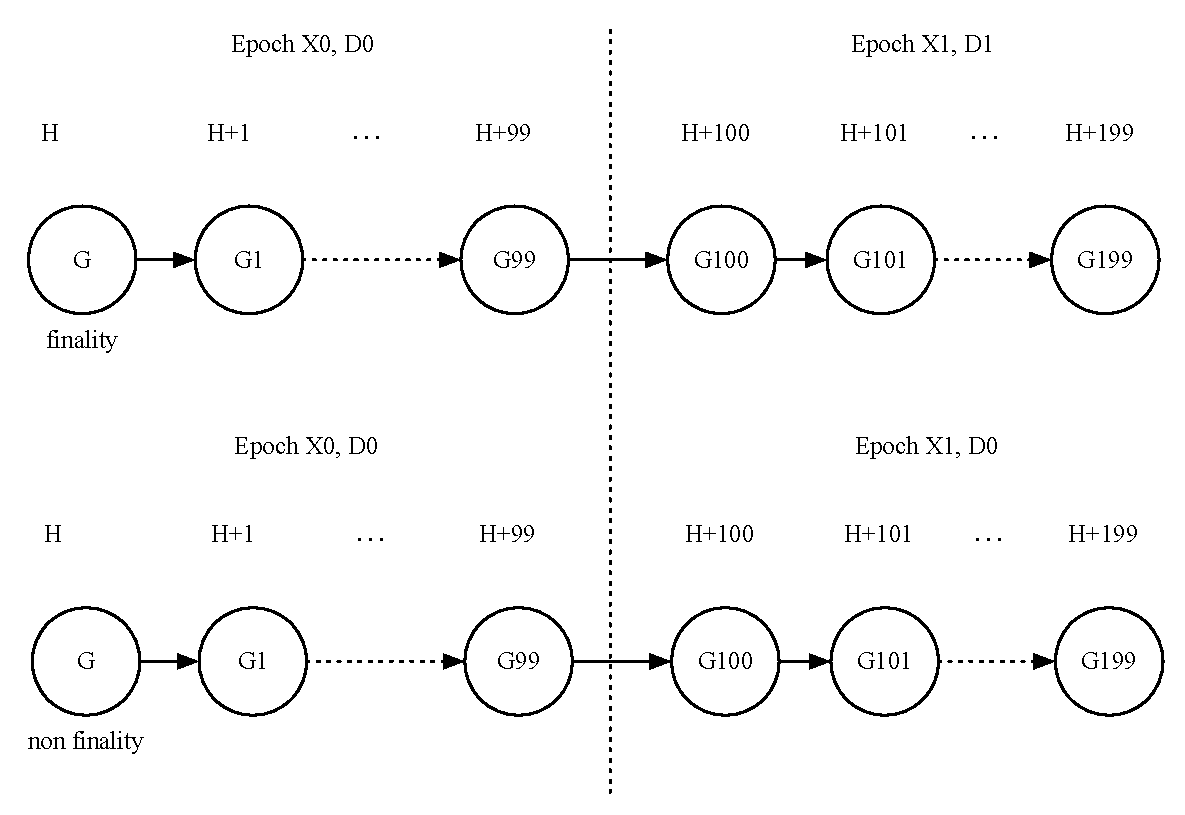
\includegraphics[width=8cm]{./figs/epoch}
\caption{Change of validator dynasties (assuming X = 100)}
\label{fig:epoch}
\end{figure}

Because of the network delay, the finality state of Block G at each node may not be the same when any change of dynasties takes place. Therefore, by reference to dynamic Casper validator set strategies, it is required that the consensus process of each dynasty will be completed jointly by the validator sets of the current and previous dynasties. Therefore, in any dynasty, an eligible account can only apply for joining or quiting the validator set of Dynasty D+2, and when the dynasty evolves into Dynasty D+2, it can participate in the consensus process of the new block.

%由于网络延迟,各个节点可能在朝代更迭时,看到的区块G是否finality的状态不一致,所以参考Casper的动态验证集策略,要求每一个朝代的共识过程将由当前朝代和上一个朝代的验证者集合共同完成。因此在任意一个朝代,有资格的账户只能申请加入或者退出D+2朝代的验证者集合,当朝代变更到D+2时,才可加入新区块的共识过程。

\subsubsection{Consensus Process}
\label{pod:design:consensus}

After a new block is proposed, all the people in the validator set of the current dynasty will participate in a round of BFT-Style (Byzantine-Fault-Tolerant Style) voting to determine the legitimacy of this block. In the beginning of voting, each validator who participates in this block consensus will be charged 2x (x is the incentive bonus proportion) as the deposit and then the two-stage voting process will be kicked off.

%新的区块被提出后,当前朝代验证者集合中所有人将会参与一轮BFT (Byzantine Fault Tolerant)方式的投票,来确定此区块的合法性。在投票最开始,每一个参与此区块共识的验证者将会被从押金中收取$2x$ ($x$为激励奖金比例)的保证金,然后进入两阶段的投票过程。

\begin{itemize}

\item \textbf{In the first stage}, it is required that all validators vote $Prepare$ tickets for the new block. After voting the $Prepare$ ticket, the validator will be rewarded $1.5x$ bonus. If the validators holding over two-thirds of the total deposits in both current and previous dynasties vote $Prepare$ tickets for the new block, this block will enter into the second stage of voting. It should be noted that the proposer of the new block votes the $Prepare$ ticket for the new block by default.

%\item \textbf{第一阶段},所有验证者需要对新区块投$Prepare$票,投完$Prepare$票的验证者将获得$1.5x$的奖励,如果在当前朝代和上一个朝代中都有超过$2/3$的押金总额的验证者对新区块投了$Prepare$票,那么该区块进入投票的第二阶段。此处需要说明,新区块的提议者将被默认对新区块投$Prepare$票。

\item \textbf{In the second stage}, it is required that all validators vote $Commit$ tickets for the new block. After voting the $Commit$ ticket, the validator will be rewarded $1.5x$ bonus again. If the validators holding over two-thirds of the total deposits in both current and previous dynasties vote $Commit$ tickets for the new block, this block will reach the finality state.

%\item \textbf{第二阶段},所有验证者需要对新区块投$Commit$票,投完$Commit$票的验证者,可以再获得$1.5x$的奖励,如果在当前朝代和上一个朝代中都有超过$2/3$的押金总额的验证者对新区块投了$Commit$票,那么该区块到达finality状态。
\end{itemize}

In order to speed up the development of the entire ecology, if the difference between the timestamp of $Prepare$ ticket and $Commit$ ticket in Block b and the timestamp of Block b exceeds $T$, then these tickets will be considered expired and will be ignored directly.

%为了加速整个生态向前延展,如果区块b的$Prepare$和$Commit$票的时间戳和区块b的时间戳相差超过T,那么这些票将被视为过期,直接忽略。

\subsubsection{Fork Choice}
\label{pod:design:fork}

The PoD algorithm selects the canonical chain according to the block score at each height. It always selects the block with the highest score to join the canonical chain, and the score of Block b at Height h is as follows:

%PoD算法以每个高度上区块的得分来选择权威链,总是选择得分最高的区块加入权威链,在高度h的区块b的得分如下,

\begin{align}
Score(b, h) = \sum_{(b',h') \in children(b)}Score(b', h') + \sum committed~deposits~in~b
\end{align}
\noindent 

Namely the sum of deposits corresponding to $Commit$ tickets received by this block and all of its descendant blocks, as shown in \reffig{fig:fork_choice}.

%即为该区块及其所有后代区块收到的commit票对应的押金总和,如图\ref{fig:fork_choice}所示。

\begin{figure}[h]
\centering
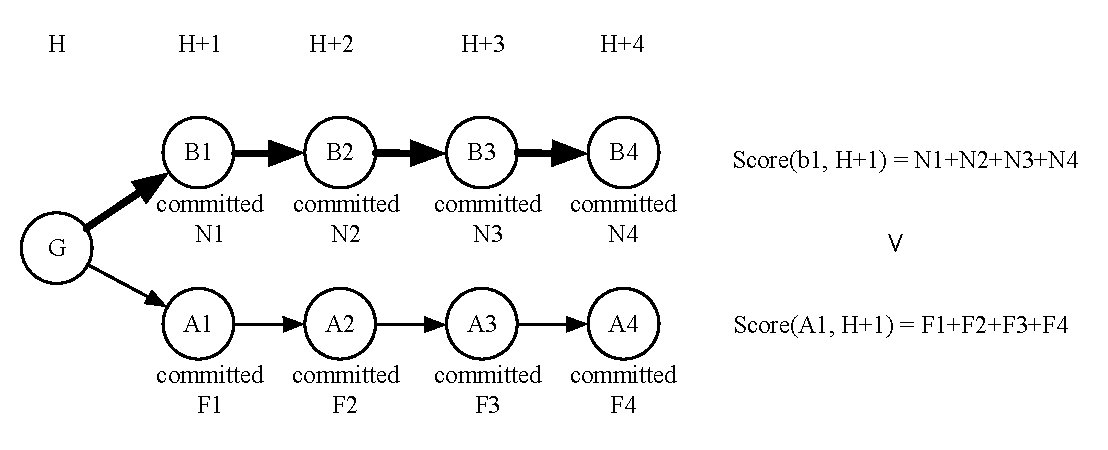
\includegraphics[width=12cm]{./figs/fork}
\caption{Fork Choice Example}
\label{fig:fork_choice}
\end{figure}

\subsubsection{Slashing Conditions}
\label{pod:design:vote}

To avoid any malicious damage to the consensus process, which may result in failure in the completion of consensus process and obstruction of eco-development, PoD constrains consensus activities of validators based on reference to Casper’s minimum slashing conditions \cite{minimal_slash_rules}.

%为了避免共识过程被恶意破坏,导致共识过程没法完成,阻碍生态发展,PoD参考Casper的最小惩罚规则~\cite{minimal_slash_rules}来约束验证者的共识活动。

Assume that $Prepare$ vote and $Commit$ vote in the consensus process have the following structures:

%假设共识过程中的$Prepare$和$Commit$票结构如下,

\begin{itemize}
\item $Prepare(H, v, vs)$, where $H$ is the hash value of the current block; $v$ represents the height of the current block; $vs$ represents the height of a certain ancestral block of $v$. 
%\item $Prepare(H, v, vs)$,其中$H$为当前区块hash,$v$表示当前区块高度,$vs$表示$v$的某个祖先区块高度

\item $Commit(H, v)$, where $H$ is the hash value of the current block; $v$ represents the height of the current block.
%\item $Commit(H, v)$,其中H为当前区块hash,$v$表示当前区块高度
\end{itemize}

PoD algorithm defines the following 4 basic rules for the entire voting process: 
%PoD算法为整个投票过程制定了如下4条基本规则,

\begin{itemize}
\item There is a strict order in the two-stage consensus process of a single block: Only when the total deposits of $Prepare(H, v, vs)$ votes for the first stage reaches $2/3$, can validators deliver $Commit(H, v)$ votes for the second stage.
%\item 单个区块的两阶段共识过程存在严格的先后顺序,只有在第一阶段$Prepare(H, v, vs)$票总权值达到$2/3$后,验证者们才可以投出第二阶段的$Commit(H, v)$票,

\item For multiple blocks, there is no mandatory rule that only when the consensus process of one block is finished, may consensus process of the next block begin. Interwoven consensus is permitted providing that it is conducted based on a certain order. Only after the first stage of process for height vs is finished and the proportion of $Prepare(H, vs, vs’)$ votes reaches $2/3$, can $Prepare(H, v, vs)$ votes for its descendant blocks be delivered based on vs in order to ensure stable proceeding of the interwoven consensus.
%\item 多区块间不强制一个区块共识结束后才能开始后一个区块的共识,允许交织共识(interwoven consensus),但是不能完全没有秩序,只有高度vs完成了第一阶段过程,拥有$2/3$的$Prepare(H_anc, vs, vs’)$后,才可以基于vs对其后代区块投$Prepare(H, v, vs)$票,保证交织稳步向前

\item To avoid the conduct of malicious cross-block voting of any node by taking advantage of the interwoven consensus, it is required that after the delivery of Prepare (H, w, u) votes based on the height of u, no Commit(H, v) vote can be delivered in all blocks with a height within the range from u to w, thus guaranteeing high efficiency and orderliness of the consensus process.
%\item 为了避免有节点利用交织共识恶意跨多区块投票,要求基于高度u投出了$Prepare(H, w, u)$票之后,对于高度在跨度u和w之间的所有区块,不能再投出$Commit(H, v)$票,保证共识过程的高效有序

\item For the purpose of preventing nodes from staking with one deposit on multiple branches simultaneously, which may lead to the problem of “nothing-at-stake”, it is required that after $Prepare(H1, v, vs1)$ votes are delivered at a certain height, no different $Prepare(H2, v, vs2)$ vote can be delivered again.
%\item 为了制止节点用同一笔押金在多个分支上同时下注,导致nothing~at~stake的问题,要求在一个高度投出$Prepare(H1, v, vs1)$票之后,不能再投出不一样的$Prepare(H2, v, vs2)$票
\end{itemize}

Once being reported and verified, any validators breaking the above rules will be punished and all his/her deposit will be confiscated, in which 4\% will be shared by whistleblowers as a reward and the remaining part will be destroyed.
%违反上述规则的验证者一旦被举报核实,将会被罚掉所有押金,举报者们将会共享罚金的4\%作为奖励,罚金的剩余部分将会被销毁。

\subsection{PoD Economic Analysis}
\label{pod:economic}

\subsubsection{Incentive Analysis}
\label{pod:economic:incentive}

A validator participating in the PoD algorithm will be rewarded with $1x$ NAS on each legal block. In case of failure in finishing the $Prepare$ stage and entering into the $Commit$ stage due to poor network traffic or any cheating behavior, the validator will lose $0.5x$ NAS. Therefore, any validator becoming value nodes will secure a large amount of earnings from accounting under good network traffic when not engaging in any cheating behavior.

%参与PoD算法的验证者,在每一个合法区块上可以获得1x的星云币奖励,如果网络不畅或者有人作弊导致Prepare阶段没有办法完成进入Commit阶段,那么所有验证者将损失0.5x。因此成为验证者的价值节点在保持网络畅通,不参与作弊的情况下,将共享大量记账收益。

\subsubsection{Cheating Analysis}
\label{pod:economic:fraud}

\subsubsection*{Double-spend Attack}
\label{pod:economic:fraud:double_spend}

If it is assumed that a merchant confirms transaction and makes delivery when the new block reaches the status of finality, then the minimum cost to be paid by a fraud for realizing zero-cost shopping through completion of double-spend attack under the PoD consensus algorithm is described as follows:

%假设商户merchant等到新区块到达finality状态就确认交易发货,那么fraud要在PoD共识算法下完成双重支付攻击实现零成本购物要付出的最小代价如下:

Firstly, the fraud needs to increase his/her Nebulas Rank to Top N, become a validator by paying a certain amount of NAS as deposit and apply for participation in validation of blocks in the D+2 dynasty. 

%首先,fraud需要提高自己的Nebulas Rank到Top N,然后缴一定数的NaS作为押金成为验证者,并申请参与D+2朝代区块的验证。

Then, the fraud needs to be selected as the proposer of a new block by the pseudo-random algorithm. At this moment, the fraud proposes two new blocks at the same height, of which one block has a hash value of hash1 and contains a transferring transaction from the fraud to the merchant, while the other block has a hash value of hash2 and contains a transferring transaction from the fraud to himself/herself. 

%然后,fraud需要被伪随机算法选中为新区块的提议者,此时fraud提出两个高度相同的新区块,一个哈希值为hash1包含fraud向merchant的转账交易,另一个哈希值为hash2包含fraud向fraud自己的转账交易。

Finally, in order to make both of hash1 and hash2 blocks reach finality, as shown in \reffig{fig:double_spend}, the fraud has to spend $1/3$ of the total deposits in this dynasty to bribe $1/3$ of the validators and make them to deliver $Commit$ votes to both blocks.

%最后,为了让hash1和hash2区块都到达finality,如图\ref{fig:double_spend}所示,fraud至少需要花费所有押金的$1/3$来贿赂$1/3$的验证者,让他们给两个区块都投$Commit$票。

\begin{figure}[h]
\centering
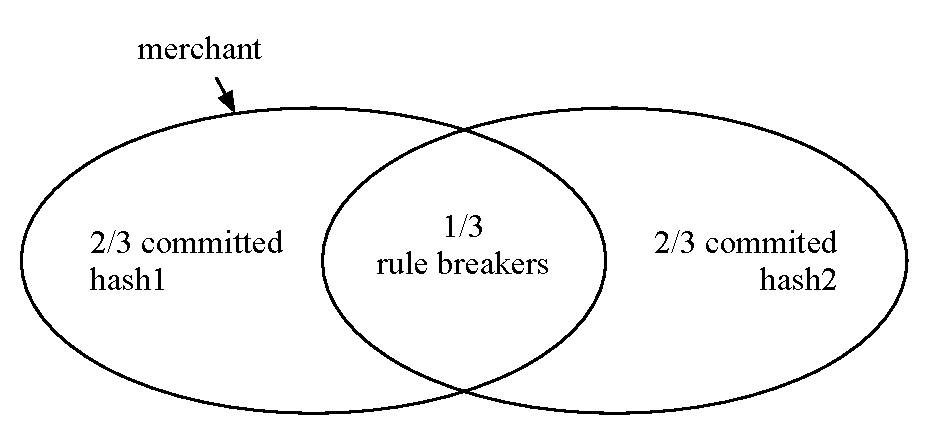
\includegraphics[width=7cm]{./figs/overlap}
\caption{Financial Punishment on Double Spend}
\label{fig:double_spend}
\end{figure}

Therefore, in order to complete a successful double-spend attack, the fraud needs to spend a certain amount of energy and financial resource to increase his/her Nebulas Rank (see \refsec{subsec:robust} Resistance to Manipulation) and then spend at least $1/3$ of the total deposits in current dynasty to make both of the blocks reach the finality status after he/she is luckily selected as a proposer.

%所以要完成一次成功的双重支付攻击,fraud需要花费一定的精力和财力来提升自己的Nebulas Rank排名(见\refsec{subsec:robust}抵抗操纵),然后等到幸运地被选为提议者时,至少花费总押金的$1/3$来让两个块同时到达finality状态。

\subsubsection*{51\% attack}
\label{pod:economic:fraud:51attack}

In PoW, launch of a 51\% attack requires 51\% of hashrate. In PoS, launch of a 51\% attack requires 51\% of deposit. However, in PoD, launch of a 51\% attack requires 51\% of accounts in the validators set, which means that a sufficient number of highly-reputed users need to rank at Top N in the Nebulas Rank and payment of a corresponding amount of deposit is required, so it will be more difficult to launch a 51\% attack in PoD.

%在PoW中要发起51\%攻击需要51\%的算力,在PoS中则需要51\%的押金,而在PoD中,则需要验证者集合中51\%的账户,这意味着拥有足够多的高声望用户进入Nebulas Rank的Top N,并且需要支付对应的押金,因此在PoD中51\%攻击将更为困难。

\subsubsection*{Short-range Attack}
\label{pod:economic:fraud:short_range_attack}

In PoD, blocks at each height have term of expiration time of consensus. Therefore, it is almost impossible to complete a long-range attack in PoD, but it is still possible to launch short-range attacks within term of expiration time.

%PoD中的每个高度上的区块都有共识有效期,如果某个高度距离最新高度超过100时,该高度的所有区块在共识过程中将被视为过期,那么这些区块上的所有新的共识活动将会被直接忽略。因此要在PoD中完成长程攻击(long-range attack)几乎不可能,但是在有效期内依旧存在发起短程攻击的可能性。

When a short-range attacker (Attacker) attempts to forge A-chain to replace B-chain to become the canonical fork when blocks at the height of H+1 are still within term of expiration time, Attacker needs to ensure that score of block A1 is higher than that of block B1. Multiple voting will be severely punished, so it will be unavoidable for Attacker to bribe validators; otherwise, it is impossible to complete a short-range attack. For the purpose of presenting the safety of the PoD consensus algorithm, the costs to be paid by Attacker in reverting different numbers of blocks are analyzed as follows.

%短程攻击者Attacker试图在高度H+1的区块还没有过期的情况下,伪造A链来替代B链成为权威链,Attacker需要让区块A1的得分比B1更高。由于多投会被严惩,所以Attacker将不可避免地要贿赂验证者,否则无法完成短程攻击。为了展现PoD共识算法的安全性,下面分别分析使不同数量的区块失效时,Attacker需要付出的代价。

If Attacker plans to revert B1, the minimum cost to be paid by Attacker is as described in \reffig{fig:revert1}, which is equivalent to a double-spend attack. If Attacker becomes the proposer of blocks at the height of H+1, then he/she has to bribe $1/3$ of the validators in Dynasty D0 and make them conduct multiple voting in order to make A1 reach finality, for which the minimum cost is $1/3$ of the total deposits.

%如果Attacker想要使B1失效,最小代价的情况如图\ref{fig:revert1},就相当一次双重支付攻击,Attacker幸运地成为了H+1高度的区块提议者,那么至少需要贿赂朝代D0中$1/3$的验证者多投使A1达到finality,最小代价为所有押金的$1/3$。

\begin{figure}[h]
\centering
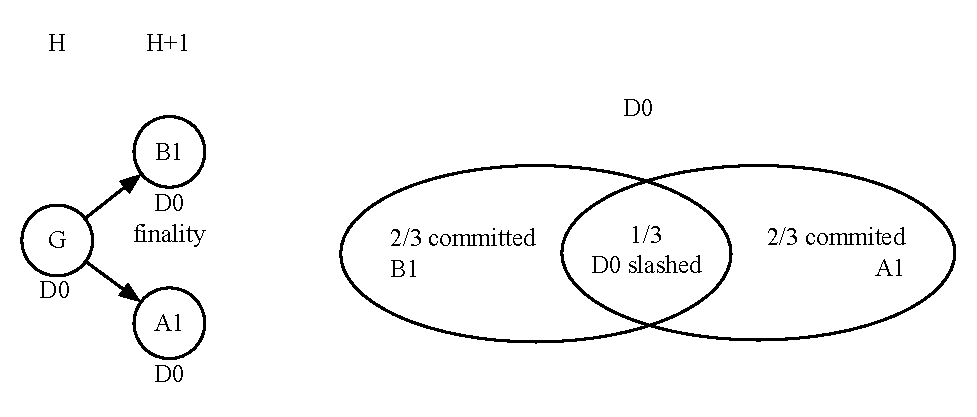
\includegraphics[width=11cm]{./figs/revert1}
\caption{Revert One Block by Short-range Attack}
\label{fig:revert1}
\end{figure}

Assume that B1 and B2 have reached the status of finality and transactions in the blocks have come into effect. If Attacker wants to revert B1-B2, the following two circumstances are taken into consideration. 

\begin{itemize}
\item The first circumstance is shown in Figure \ref{fig:revert2} (a): When Heights H+1 and H+2 are in the same Epoch and dynasty, Attacker needs to bribe $1/3$ of the validators in D0 in order to make A1 reach finality. Meanwhile, these $1/3$ of the validators will be punished and their deposits will be totally confiscated. During validation of A2, sum of deposits equals to $2/3$ of deposits in A1. At this moment, if Attacker wants to secure the same amount of commit votes as B2, he/she has to bribe all the remaining validators without cheating and lose at least $3/3$ of the total deposits. Even if Attacker succeeds in doing this, it is impossible to guarantee that score of A1 is higher than that of B1 and Attacker will face a high risk of failure of attack. 

\item The second circumstance is shown in Figure \ref{fig:revert2} (b): When Heights H+1 and H+2 are in different Epochs and different dynasties, Attacker needs to bribe $1/3$ of the validators in D0 to make A1 reach finality and then bribe $1/3$ of the validators in D1 to make A2 reach finality, so Attacker will lose at least $2/3$ of the total deposits in order to complete such an attack. To sum up, to launch a short-range attack to cause invalidation of two blocks that have reached finality, Attacker needs to pay at least $2/3$ of the total deposits. 
\end{itemize}
%如果Attacker想要使B1-B2失效,假设B1和B2都已到达finality,块中交易都已生效,为了让这些交易失效,这里考虑两种情况。第一种如图\ref{fig:revert2}中(a)所示,高度H+1和H+2在同一个Epoch中,朝代相同,那么Attacker首先需要贿赂D0中$1/3$的验证者使A1达到finality,此时这$1/3$的验证者将会被惩罚,押金被罚完。在A2的验证中整体押金总和只有A1中的$2/3$,此时Attacker想要让A2到达和B2同价值的committ票,需要贿赂剩下所有没有作弊的验证者,合起来至少需要损失总押金的$3/3$,即使如此也不能保证A1得分比B1高,攻击失败风险高。第二种情况如图\ref{fig:revert2}中(b)所示,高度H+1和H+2正好在不同的Epoch中,且朝代不相同,那么此时Attacker需要贿赂D0中的$1/3$来让A1到达finality,然后贿赂D1中的$1/3$来让A2达到finality,完成一次这样的攻击至少需要损失总押金的$2/3$。综上,想要发起短程攻击导致两个finality区块失效,至少需要花费总押金$2/3$的代价。

\begin{figure}[h]
\centering
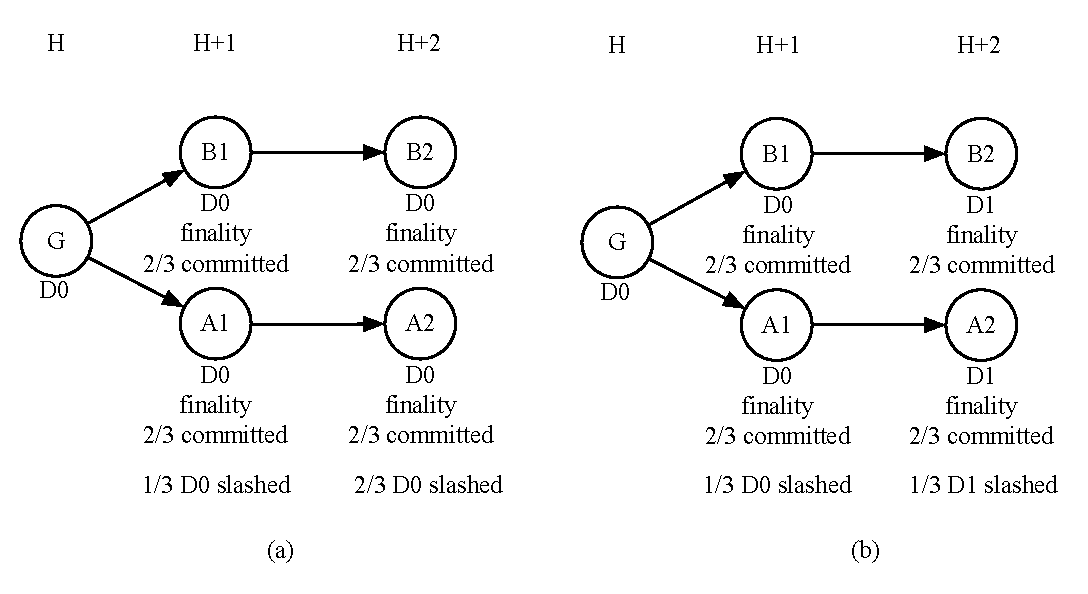
\includegraphics[width=11cm]{./figs/revert2}
\caption{Revert Two Blocks by Short-range Attack}
\label{fig:revert2}
\end{figure}

If Attacker wants to revert B1-B3, as shown in Figure 18, Attacker needs to firstly bribe $1/3$ of the validators in D0 in order to realize finality of A1 and then bribe $1/3$ of the validators in D1 in order to realize finality of A2. Finally, Attacker needs to bribe all of the remaining $2/3$ of the validators in D1 in order to realize finality of A3. To sum up, $4/3$ of the total amount of deposits will be lost. It will be very difficult to prepare for these attacks. Even if an attacker manages to succeed in making necessary preparations, he/she can’t guarantee that score of A1 is higher than that of B1. Therefore, it is possible that such attack may fail.

%如果Attacker想要使B1-B3失效,如图\ref{fig:revert3}所示,Attacker首先需要贿赂D0中$1/3$的人完成A1的finality,然后贿赂D1中$1/3$的人完成A2的finality,最后需要贿赂D1中剩下$2/3$中的所有人来完成A3的finality,综上至少要损失总押金的$4/3$。要完成这些攻击准备将会十分困难,而且即使有幸做到了,也不定能保证A1的得分比B1高,攻击也可能会失败。

\begin{figure}[h]
\centering
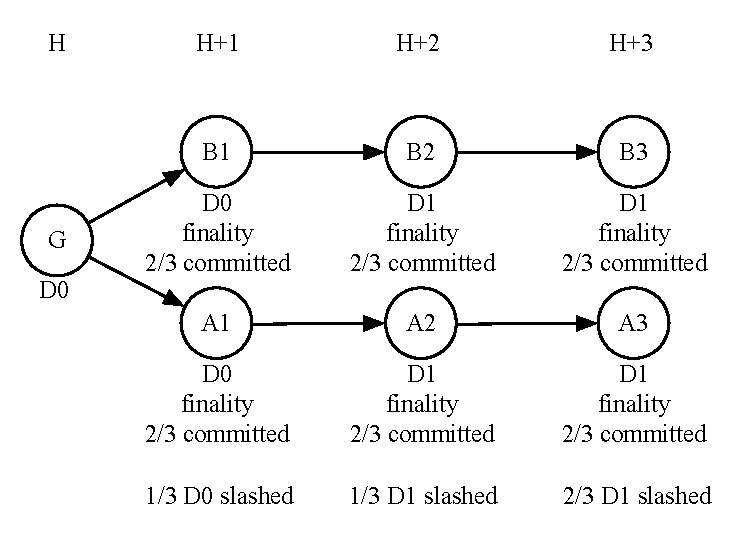
\includegraphics[width=7.5cm]{./figs/revert3}
\caption{Revert Three Blocks by Short-range Attack}
\label{fig:revert3}
\end{figure}

If Attacker wants to revert B1-BN, in which N is limited by term of expiration time of consensus of the block and thus can't be a very large number. When $N = 3$, the total deposits of all validators in the current dynasty will be totally confiscated. Therefore, when $N >= 4$, it is impossible to complete an attack in order to make score of B1 higher than that of A1 and revert B1-BN. It is pointless to launch such an attack.

%如果Attacker想要使B1-BN失效,其中N受到区块共识有效期的限制,不会很大,由于$N=3$时当前朝代所有验证者的押金就会被全部罚完,所以$N>=4$时,将没法完成攻击让B1得分比A1高,使B1-BN失效,发起这样的攻击没有任何意义。
